\newpage
\section{Anonymisering av bilder med ansikter}
\label{sec:Anonymisering}
\subsection{Bakgrunn}
Anonymisering av bilder er enkelte ganger nødvendig før det blir offentlig vist frem for å skjerme den avbildedes personvern. En teknikk som ofte blir brukt er å gjøre ansiktene uskarpe mens resten av bildet forblir skarpt. Teknikken avhenger av at programmet klarer å gjenkjenne ansiktene\cite{wiki:FaceDetection} for å definere en maske rundt, slik at man kan isolere anvendingen av bildet kun på ansiktet. I denne oppgaven brukte vi biblioteket OpenCV (Open Source Computer Vision Library) og maskinlæringsalgoritmen Haar Cascade. 

\subsubsection{Open CV}
Open CV er et open source datasyn-\cite{datasyn} og maskinlæringsbibliotek som ble utviklet for å skape en felles infrastruktur for datasynsapplikasjoner og for å akselerere bruken av maskinoppfatning i kommersielle produkter\cite{cv2}. Kort fortalt betyr dette datamaskinens evne til å tolke data på en måte som ligner på hvordan mennesker bruker sansene til å oppfatte verden rundt seg, og da spesielt synet i dette tilfellet. Gjennom dette biblioteket kunne vi implementere Haar Cascade algoritmen til å gjenkjenne ansikter

\subsubsection{Haar Cascade algoritmen}
Haar Cascade er en maskinlæringsalgoritme~\cite{haar} som brukes til å identifisere objekter i et bilde eller i en video. Den er mest kjent for å identifisere ansikter, men kan trenes til å identifisere diverse andre ting. Alt ettersom den blir trent riktig.

Algoritmen trenger må trenes med flere positive bilder av ansikter og negative bilder uten ansikter, deretter må man trekke ut kjente ansiktstrekk fra disse bildene. Første steget er å samle inn Haar-features. 

\begin{figure}[H]
\begin{center}
    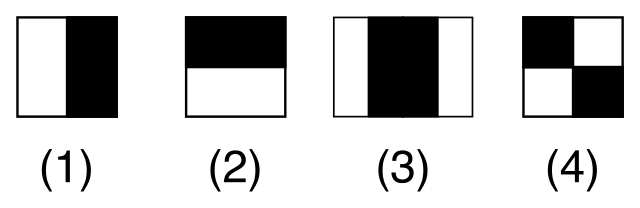
\includegraphics[width=0.4\columnwidth]{bilder/Anonymisering/VJ_featureTypes.svg.png}
     \caption{Haar Features\label{fig:haarfeat}} \source{Wikimedia Commons~\cite{wiki:haarfeat}}
\end{center}
\end{figure}

De to første elementene (figur \ref{fig:haarfeat}) kalles for edge-features som benyttes til å oppdage kanter. Den tredje er en line-feature, mens den fjerde heter four rectangle-feature som oftest benyttes til å gjengkjenne en skrå linje. Edge-features klarer å gjengkjenne essensielle deler ved et ansikt, som f.eks et øye. Grunnen til dette er at i bildet blir det en kontrast mellom øyet og kinnet, som kan minne om objekt 2 fra figur \ref{fig:haarfeat}, altså en mørk overdel med lys bunn. Algoritmen går så gjennom hele bildet systematisk helt til det oppdager en samling av slike ``features'' og ved nok positive treff markerer den det område som et ansikt.

Algoritmen trenger to parametre, nemlig scale factor og nearest neighbour. Økes scale factor økes også ytelsen, fordi antall passeringer over bildet blir redusert, men dette er et bytte mot at påliteligheten blir dårligere. Altså at den vil gjøre feil i gjenkjenningene. Riktig scale factor avhenger av bildet, men en verdi på 1.2 gir som regel en pålitelig gjenkjenning. Man er nødt til å vurdere verdien på scale factor hvis enkelte ansikter er lengre bak enn andre på bildet. Altså hvis noen ansikter fremstår større ut, så vil algoritmen ta feil hvis ikke parametrene blir justert i henhold.

Den andre parameteren; minimum neighbour definerer antall nærliggende ansiktstrekk som er nødvendig for at programmet skal akseptere det som et ansikt. På samme måte så er det lurere å ha et høyt tall her hvis ansiktene er rimelig store på bildet, siden hvert ansiktstrekk blir mer detaljert. det anbefales et sted mellom 3 og 5 for at man skal oppnå best resultat på de aller fleste bilder. Resultatet av implementasjonen vises i figur \ref{fig:science}
\begin{figure}[H]
\begin{center}
 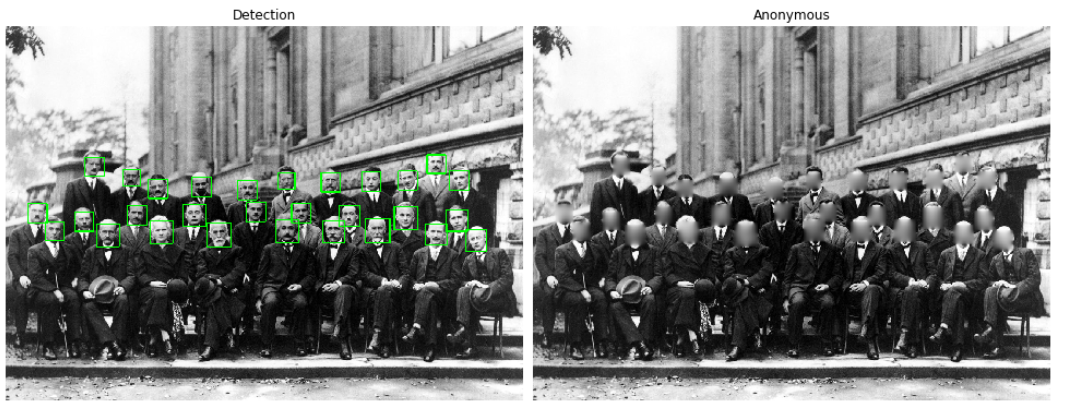
\includegraphics[width=1\columnwidth]{bilder/Anonymisering/faceDetectionExample.png}
     \caption{Eksempel på anonymisering \label{fig:science}} \source{Wikimedia Commons~\cite{wiki:science}}
\end{center}
\end{figure}

\subsection{Implementasjon}
Det mest krevende med implementasjonen var å få programmet til å gjenkjenne ansikter. Viktigste var å importere xml-filen\footnote{haarcascade\_frontalface\_default.xml\cite{xml:haar}} som inneholdt en ferdig trent algoritme for gjenkjenning av ansikter som er vendt direkte mot kamera. Neste steg var å tegne rektangel rundt område der algoritmen gjenkjente som ansikt. Etter dette var det bare å trekke ut det oppdagede ansiktet som en maske $\Omega_i$ også løse ligning~(\ref{eq:diffusjon}) med $h=0$ i $\Omega_i$ og med Dirichlet-betingelsen $u = u_0$ på $\partial\Omega_i$.
\begin{lstlisting}[language=Python]

def blurFace(file, scaleFactor = 1.2, minNeighbors = 5):
image = cv2.imread(file)                            # leser inn bildet BGR
    image = cv2.cvtColor(image, cv2.COLOR_BGR2RGB)  # konverterer til RGB
    
    face_cascade = cv2.CascadeClassifier('Resources/haarcascade_
                                         frontalface_default.xml') 
    faces = face_cascade.detectMultiScale(image, scaleFactor, minNeighbors)
                                        
    for (x,y,w,h) in faces:             # For alle ansiktene funnet
        RoI = image[y:y+h, x:x+w]       # Region of Interest
        RoI = RoI.astype(dtype = float)
        blur = eks.eksplisittDirichlet(RoI,image[y:y+h, x:x+w], 0.25,250)               
        image[y:y+h, x:x+w] = blur
        
    return len(faces), image    #Returnerer antall ansikt og anonymt bilde
\end{lstlisting}

\begin{lstlisting}[language=Python]
-------------------------------------------------------------------------
def eksplisittDirichlet(u,u_0, alpha=0.25, n=1000):
    for i in range(n):                      # Itererer n antall ganger
        u[1:-1, 1:-1] += alpha * (u[:-2, 1:-1] + u[2:, 1:-1]
                      + u[1:-1, :-2] + u[1:-1, 2:] - 4 * u[1:-1, 1:-1])
        u[0] = u_0[0]  
        u[-1] = u_0[-1]                     # Dirichlet randbetingelser
        
    return u
\end{lstlisting}


